\section{Cape of Good Hope - Postal History } 
\section{Stamp Booklet}
The Cape of Good Hope post office only issued one booklet with the King Edward VII stamps in panes of six (30 stamps in all Value 2s 7d). The extra 1d was charged to offset the cost of the booklet. These booklets were issued towards the end of 1905.

\begin{figure}[htbp]
\centering
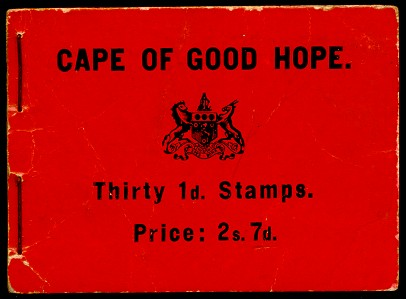
\includegraphics[width=.60\textwidth]{../cape-of-good-hope/stamp-booklet.jpg} 
\caption{Booklet 1905 KEVII 2/7 Rare. SG SB1}
\end{figure}

The inside of the front cover had details of Inland Postage rates. The inside of the back cover had foreign postage information, while the outside had information on
Telegrams. Apparently half the booklets were stapled at left and half stapled at right.

Very few booklets have survived so it is extremely difficult to find information on them.\footnote[]{tests}

\subsubsection{References}
1. Trotter Brian, Cape of Good Hope Edwardian Postage Stamps, \textit{London Philatelist}, July/August 2001, \textbf{110}:198.





1287.pdf



	 
                                    